
\documentclass{IOS-Book-Article}

\usepackage{mathptmx}
\usepackage{subcaption}
\usepackage{times}
\usepackage{CJKutf8}
\usepackage{mathrsfs}
\usepackage{textcomp}
\usepackage{verbatim}
\usepackage{amsmath}
\usepackage{amsfonts}
\usepackage{xspace}
\usepackage{xcolor}
\usepackage{url}
\usepackage{balance}
\usepackage{booktabs}
\usepackage{multirow}
\usepackage{rotating}
\usepackage{fancyvrb}
\usepackage{lastpage}
\usepackage{alltt}
\usepackage{etoolbox}
\usepackage{cleveref} % After hyperref, listings
\usepackage{fancyhdr}
\usepackage{listings}
\usepackage{caption}

%\usepackage{times}
%\normalfont
%\usepackage[T1]{fontenc}
%\usepackage[mtplusscr,mtbold]{mathtime}
%
\def\hb{\hbox to 10.7 cm{}}

\begin{document}

\pagestyle{headings}
\def\thepage{}

\begin{frontmatter}              % The preamble begins here.


%\pretitle{Pretitle}
\title{Optimizing CPU Performance and Scalability of Google Tensorflow for
Manycore CPU}
%\markboth{}{September 2016\hb}
%\subtitle{Subtitle}
%\author[A]{\fnms{Book Production} \snm{Manager}%
%\thanks{Corresponding Author: Book Production Manager, IOS Press, Nieuwe Hemweg
% 6B, 1013 BG Amsterdam, The Netherlands; E-mail:
%bookproduction@iospress.nl.}},
%\author[B]{\fnms{Second} \snm{Author}}
%and
%\author[B]{\fnms{Third} \snm{Author}}

%\runningauthor{B.P. Manager et al.}
%\address[A]{Book Department, IOS Press, The Netherlands}
%\address[B]{Short Affiliation of Second Author and Third Author}

\begin{abstract}
We propose a optimization method for Google Tensorflow on a single shared-memory
manycore architecture using new CPU optimizing and efficient memory placement
methods to improve performance scalability.
The performance problems of Tensorflow frameworks have only considerd on large
distributed clusters of CPUs and GPUs resulting from the cluster-based
algorithms that focused on avoiding high network costs and improving GPU
performace.
However, some of large scale machine learning data can be proccesed with a
single commodity manycore machine instead of using distributed clusters
with GPUs since shared memory systems can reduce network and PCI-E bus
transfers.
The proposed methods can improve performance and scalability on the
unoptimized Tensorflow on a single manycore machine by using efficient
vectorization, maximizing CPU utilization and efficient memory placement.
Our preminerly method will provide the basis towards practical
design of deep learing framework for a single manycore server to collaborate
CPUs and GPUs.
Our evaluation study based on benchmark programs revealed that the our
optimizing method will show better performance improvement through on a 64
core Intel Xeon-phi KNL, self-bootable single manycore CPUs, compared to
unoptimized Tensorflow.
\end{abstract}

\begin{keyword}
Mayncore\sep Tensorflow\sep Intel Xeon-phi\sep 
\end{keyword}
\end{frontmatter}
%\markboth{September 2017\hb}{September 2016\hb}
%\thispagestyle{empty}
%\pagestyle{empty}


\section{Introduction}
In recent years, deep learning has produced several domains ranging from speech
recognition, visual object recognition, to text processing.
However, deep learning data sets have substantially grown during the last
decade. 
To solve large data sets, the current design trend is to use large-scale
clusters of machines to distribute training and inference in deep networks
using deep learning frameworks.
Google Tensorflow~\cite{Abadi2016TSL} is one of widely used deep learning
analytics framework to solve large data sets problem, and it becomes more and more versatile
framework for distributed clusters, local workstations, mobile devices, and
custom-designed accelerators.
However, Tensorflow does not scale on the single manycore machine
resulting from our preminerly expermiments(Section x) because Tensorflow was
the successor to DistBelief~\cite{Dean2012LSD}, a heavyweight system, and it
only added support for GPU acceleration~\cite{Abadi2016TSL}.

Alexander Matveev., et,al. proposed a deep learning algorithm and CPU optimizing
methods that eliminate the bottleneck of transferring data to the cloud thereby
reducing the overheads from a large cluster to a single commodity
multicore server~\cite{Matveev2017MPC}.
We also believed that some workloads on a single manycore machine can perform
faster than a distributed clusters of CPUs and GPUs.
Thus, CPU scaling problem on single manycore server must be resolved on
Tensorflow.
Our new method will provide the basis towards practical design to collaborate
CPUs and GPUs.

\begin{figure*}[tb]
    \centering
    \begin{subfigure}[b]{0.5\textwidth}
        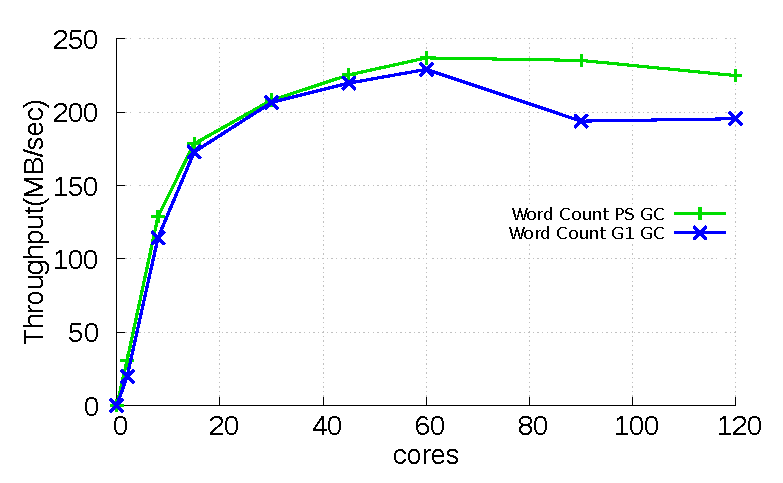
\includegraphics[width=2.3in]{graph/wc.eps}
        \caption{Scale-up server scalability of Caffe}
    \end{subfigure}%
    \begin{subfigure}[b]{0.5\textwidth}
        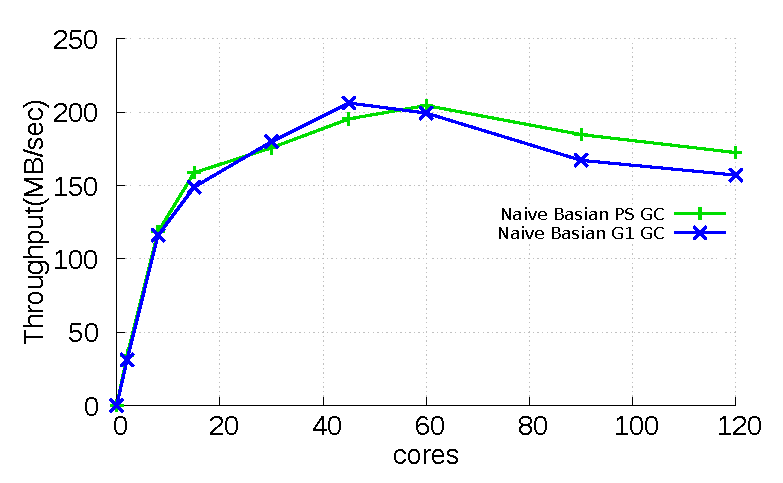
\includegraphics[width=2.3in]{graph/nb.eps}
        \caption{Scale-up server scalability of Tensorflow}
    \end{subfigure}%
    \label{fig:docker}
\end{figure*}


\section{Preminerly Expermiments}
As noted earlier, Tensorflow does not scale on the single manycore machine.
In order to achieve the high performance on Tensorflow, we need to understand 
the problme of Tensorflow on a single manycore machine.
The figure x-x explains the improving point of original Caffe on Intel Xeon-phi
KNL;original Caffe didn't scale well.
On the other hand, Intel optimized Caffe on Intel xeon-phi KNL processor.
However, until recently, figure x-x shows that Tensorflow has not been 
optimized on Intel xeon-phi KNL processor due to the it does not support CPU
optimizationg technique such as OpenMP and Intel MKL libarys.
This resualts show us to problem of performance and scalability on a single
manycore machine.

\section{Proposed Methods}
In order to achieve the high performance on Tensorflow, we may use a method 
to avoid the major drawbacks of the Tensorflow regarding utilizing all the
core, vectorizing, efficient memory access.
Our proposed architecture is based on the reasoning that logically partitioning
the original servers into small servers could hide the Spark's performance
scalability problems.
 
\bibliographystyle{abbrv}
\bibliography{ref}
 
%\begin{thebibliography}{99}
%\bibitem{r1}
%\textit{Scientific Style and Format: The CBE manual for authors,
%editors and publishers}. Style Manual Committee, Council of Biology Editors.
%Sixth ed. Cambridge University Press, 1994.

%\bibitem{r2}
%L.U. Ante, Cem surgere: Surgite postquam sederitis, qui manducatis panem
% doloris, \textit{Omnes} \textbf{13} (1916), 114--119.

%\bibitem{r3}
%T.X. Confortavit, \textit{Seras}, Portarum, New York, 1995.

%\bibitem{r4}
%P.A. Deus, Ater hoc et filius et mater praestet nobis,
%\textit{Paterhoc} \textbf{66} (1993), 856--890.

%\end{thebibliography}

\end{document}
